\section{Critical values}\label{sec:cv}

\begin{figure}[tbp]\centering
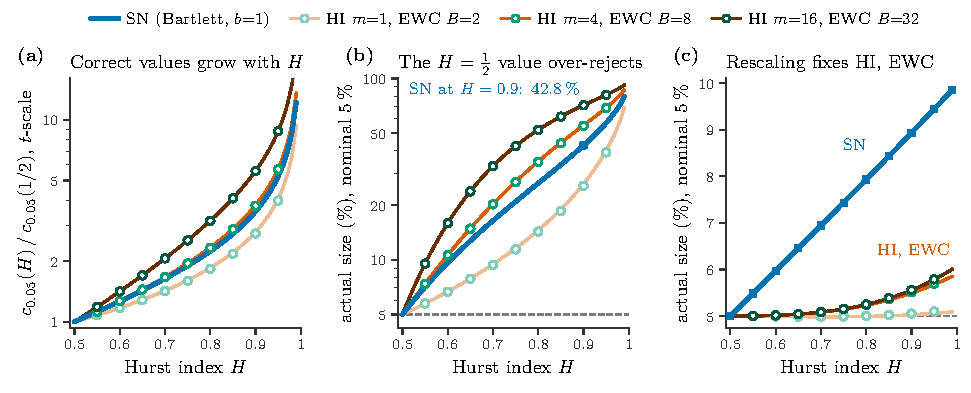
\includegraphics[width=\textwidth]{fig1_headline.pdf}
\caption{Critical values and limit size of the three test families. (a)~Two-sided $5\,\%$ critical values relative
to short-memory values ($t$ scale). (b)~Limit size of nominal $5\,\%$ tests using short-memory values.
(c)~As (b) after the rescaling of \cref{prop:rho} (narrower vertical range). Lines: HI, $m$ frequencies;
circles: EWC, $B=2m$; all values certified.}\label{fig:headline}
\end{figure}

\subsection{The Bartlett/self-normalised statistic}
\Cref{tab:sncv} gives the quantiles of $T_H$ for selected $H$; \cref{app:tables} gives all
\pthree{sn-n-H} values $H=0.50,0.51,\dots,0.99$ at the six levels $p\in\{0.80,0.90,0.95,0.975,0.98,0.99\}$, which cover
two-sided tests at $10$, $5$ and $1\,\%$ and one-sided tests with the signed statistics at $10$, $5$, $1.25$ and $1\,\%$.
A two-sided test at level $\alpha$ rejects when $T_n>q_{1-\alpha}$; a one-sided test at level $a$ with the signed
statistic $t$ of \citet{KV02} or \citet{MP12} ($T_H=2t^2$) rejects when $t>\sqrt{q_{1-2a}/2}$, and with the statistic of
\citet{KVB00} ($T_H=t^2$) when $t>\sqrt{q_{1-2a}}$.
Each value carries a certified enclosure: the largest relative half-width over the \pthree{sn-n-cells} cells is
\pthree{sn-max-relwidth}, attained at $H=\frac12$, and every printed value is the correctly rounded value of every number
in its enclosure. At $H=\frac12$
the values agree with the closed-form law of \citet{AP97} to \pthree{g0-min-digits} significant digits or more.

\begin{table}[tbp]\centering\small
\caption{Certified quantiles $q_p(H)$ of $T_H$; each entry is correctly rounded, so the number of digits varies.}\label{tab:sncv}
\begin{tabular}{@{}lrrrr@{}}\toprule
$H$ & $q_{0.80}$ & $q_{0.90}$ & $q_{0.95}$ & $q_{0.99}$\\\midrule
0.50 & 15.015 & 28.331 & 45.53 & 100.3\\
0.55 & 18.450 & 35.23 & 57.23 & 128.9\\
0.60 & 22.876 & 44.195 & 72.555 & 166.84\\
0.65 & 28.726 & 56.144 & 93.147 & 218.70\\
0.70 & 36.7212 & 72.6087 & 121.741 & 291.854\\
0.75 & 48.1606 & 96.3545 & 163.284 & 399.760\\
0.80 & 65.6455 & 132.920 & 227.701 & 569.48\\
0.85 & 95.2468 & 195.244 & 338.197 & 864.40\\
0.90 & 155.181 & 322.168 & 564.474 & 1475.24\\
0.95 & 336.540 & 707.966 & 1255.25 & 3356.71\\
0.99 & 1793.35 & 3814.26 & 6829.94 & 18613.1\\
\bottomrule\end{tabular}
%
\end{table}

The values grow quickly with memory: $q_{0.95}$ is multiplied by \pthree{sn-infl-0.80-0.950} between $H=\frac12$ and
$H=0.8$ and by \pthree{sn-infl-0.99-0.950} up to $H=0.99$. On the $t$ scale of \cref{fig:headline}a, where the
Bartlett/self-normalised value is shown as $\sqrt{q_{0.95}(H)/q_{0.95}(\frac12)}$, this is a factor
\pthree{sn-tinfl-0.99-0.950}.

\subsection{Fixed-smoothing statistics}
The fixed-$m$ and EWC limits are finite-dimensional, so their quantiles can be certified at every $0<H<1$
(\cref{prop:continuation}). \Cref{tab:fixedcv} gives two-sided $5\,\%$ values; \cref{app:tables} gives the
\pthree{fx-n-cells} certified values for $m=1,\dots,16$, $B\in\{1,2,3,4,6,8,12,16,24,32\}$, $\alpha\in\{0.10,0.05,0.01\}$
and $H=0.50,0.51,\dots,0.99$. At $H=\frac12$ every enclosure contains the Student-$t$ value with $2m$ or $B$ degrees of
freedom, which validates the computation against an independent closed form.

\begin{table}[tbp]\centering\small
\caption{Two-sided $5\,\%$ critical values of the fixed-$m$ statistic $\tau$ of \citet{HI17} and of the EWC statistic
of \citet{LLSW18} (certified). At $H=\frac12$ the values are $t_{2m,0.975}$ and $t_{B,0.975}$.}\label{tab:fixedcv}
\begin{tabular}{@{}lrrrrrrrrrr@{}}\toprule
 & \multicolumn{5}{c}{HI, $m$} & \multicolumn{5}{c}{EWC, $B$}\\\cmidrule(lr){2-6}\cmidrule(l){7-11}
$H$ & 1 & 2 & 4 & 8 & 16 & 2 & 4 & 8 & 16 & 32\\\midrule
0.50 & 4.3027 & 2.7764 & 2.3060 & 2.1199 & 2.0369 & 4.3027 & 2.7764 & 2.3060 & 2.1199 & 2.0369\\
0.60 & 5.0406 & 3.3665 & 2.9219 & 2.8287 & 2.8790 & 5.0366 & 3.3639 & 2.9203 & 2.8278 & 2.8785\\
0.70 & 6.1325 & 4.2418 & 3.8430 & 3.9070 & 4.1964 & 6.1039 & 4.2278 & 3.8350 & 3.9023 & 4.1937\\
0.80 & 7.9547 & 5.6995 & 5.3800 & 5.7228 & 6.4550 & 7.8712 & 5.6595 & 5.3569 & 5.7089 & 6.4466\\
0.90 & 11.978 & 8.8891 & 8.7220 & 9.6670 & 11.386 & 11.767 & 8.7863 & 8.6618 & 9.6299 & 11.363\\
0.95 & 17.517 & 13.228 & 13.221 & 14.933 & 17.933 & 17.139 & 13.042 & 13.111 & 14.864 & 17.889\\
0.99 & 40.278 & 30.842 & 31.269 & 35.829 & 43.650 & 39.276 & 30.343 & 30.970 & 35.640 & 43.529\\
\bottomrule\end{tabular}
%
\end{table}

The columns for HI with $m$ frequencies and EWC with $B=2m$ cosines are close at every $H$, although the two
self-normalisers use different coordinates (\cref{prop:coords}b); the same near-equality holds for power
(\cref{sec:power}).

\subsection{The price of the short-memory critical value}
\Cref{fig:headline}b shows the exact limit size of the nominal $5\,\%$ tests that keep the short-memory value. At $H=0.7$
the Bartlett/self-normalised test rejects a true null \pthree{naive-sn-0.70-0.05}\,\% of the time and at $H=0.9$
\pthree{naive-sn-0.90-0.05}\,\%. The fixed-smoothing tests are worse, and they are the worse the more components their
variance estimator has: at $H=0.9$ the size is \pthree{naive-hi1-0.90}\,\% for $m=1$ and \pthree{naive-hi16-0.90}\,\%
for $m=16$. The variance estimators that use more frequencies average periodogram ordinates further from the origin,
whose expectation is smaller under long memory, and they also have smaller critical values.

The same comparison can be made on data of a fixed length, where no limit argument is involved. \Cref{tab:matched} holds
the data model and the sample size fixed (fractional Gaussian noise, $n=64$ and $128$) and changes only the critical value
of the squared statistic $T_n$. With the Brownian value $45.526$ the exact size is
\pthree{mx-0.90-128}\,\% at $H=0.9$ and \pthree{mx-0.99-128}\,\% at $H=0.99$ for $n=128$; with the certified value
\pthree{mx-cv-0.99} for $H=0.99$ it is \pthree{mx-0.99-128-own}\,\%. Under long memory the finite-grid sizes differ from
the certified limit sizes by at most \pthree{mx-gap-64-long}\,pp at $n=64$ and \pthree{mx-gap-128-long}\,pp at $n=128$;
the largest gap, \pthree{mx-gap-64}\,pp, is the short-memory one at $H=\pthree{mx-gap-64-H}$ and $n=64$. For fractional
Gaussian noise the limit critical values therefore already apply at these sample sizes. The
entries are exact finite-dimensional laws, computed twice, by the series of \cref{prop:exactn} and by an independent
Imhof integral at $30$ digits, which agree to \pthree{mx-maxdiff-AB}\,pp; they also reproduce an independent
double-precision check to the printed digits (largest difference \pthree{mx-maxdiff-user}\,pp).

\begin{table}[tbp]\centering\small
\caption{Exact size (\%) under fractional Gaussian noise of the test that rejects when $T_n$ exceeds the stated value;
finite-$n$ columns are exact laws (\cref{prop:exactn}), the last column the certified limit.}\label{tab:matched}
\begin{tabular}{@{}llrrr@{}}\toprule
& & \multicolumn{2}{c}{exact, finite grid} & limit\\\cmidrule(lr){3-4}\cmidrule(l){5-5}
$H$ & critical value used & $n=64$ & $n=128$ & certified\\\midrule
0.50 & $H=\frac12$ value $45.526$ & 5.0167 & 5.0042 & 5.0000\\
0.90 & $H=\frac12$ value $45.526$ & 42.8085 & 42.8081 & 42.8080\\
0.99 & $H=\frac12$ value $45.526$ & 79.5227 & 79.5227 & 79.5227\\
0.99 & rounded certified value $6829.9$ & -- & 5.00008 & 5.0000\\
0.99 & certified value $6829.9404$ & -- & 5.00004 & 5.0000\\
\bottomrule\end{tabular}
%
\end{table}

\subsection{Why the critical values grow: collapse of the self-normaliser}\label{sec:collapse}
As $H\uparrow1$ the fractional Brownian path becomes linear, $\E|B_H(r)-rB_H(1)|^2\to0$ uniformly in $r$, so every
self-normaliser in \eqref{eq:limits} tends to zero while the numerator keeps unit variance. The rate is explicit.

\begin{proposition}[First moments of the self-normalisers]\label[proposition]{prop:rho}
Let $0<H<1$ and, for each procedure $P$, let $\rho_P(H)=\E D_P/\E_{1/2}D_P$. Then
\begin{gather*}\rho_{\SN}(H)=\frac{6}{(2H+1)(H+1)}-1,\qquad \rho_{\EWC,B}(H)=\frac1B\sum_{j=1}^BG_{jj},\\
\rho_{\HI,m}(H)=\frac1{2m}\sum_{j=1}^m\big(G_{2j,2j}+\Cov(\Sigma_{2j},\Sigma_{2j})\big),\end{gather*}
with the entries of \cref{prop:coords}. Each $\rho_P$ is real-analytic on $(0,1)$, equals $1$ at $H=\frac12$, and
$\rho_P(H)\to0$ as $H\uparrow1$; in particular $\rho_{\SN}(H)=\frac76(1-H)+O((1-H)^2)$.
\end{proposition}

The first moment alone does not determine how fast the critical values grow; the whole self-normaliser does, and it
collapses at rate $1-H$.

\begin{proposition}[Growth as $H\uparrow1$]\label[proposition]{prop:edge}
Let $\varphi(x)=x^2\log x$ ($\varphi(0)=0$) and
$k_1(r,s)=\varphi(|r-s|)-\varphi(r)-\varphi(s)+s\{\varphi(r)-\varphi(1-r)\}+r\{\varphi(s)-\varphi(1-s)\}$, which is
$-\partial_H\Cov(\Bt(r),\Bt(s))$ at $H=1$. As $H\uparrow1$, $(1-H)\,T_H\Rightarrow Z^2/\!\int_0^1G^2$, where $G$ is a
centred Gaussian process with covariance $k_1$, independent of $Z$, and $\int_0^1\E G(r)^2\dd r=\frac7{36}$. Hence
$(1-H)\,q_p(H)\to C_p$, the $p$-quantile of $Z^2/\!\int_0^1G^2$, for every $0<p<1$. The same holds for $\tau_{H,m}^2$
and $t_{H,B}^2$, for every $m\ge1$ and $B\ge1$, with the corresponding quadratic form in $G$; in particular
$\lim_{H\uparrow1}\rho_{\EWC,B}(H)/(1-H)\ge h_B/B$ and $\lim_{H\uparrow1}\rho_{\HI,m}(H)/(1-H)\ge h_m/(4m)$, where
$h_j=\sum_{i\le j}1/i$.
\end{proposition}

Numerically (a Nystr\"om discretisation of $k_1$ and Imhof's inversion; computed, not certified),
$C_{0.90}=\pthree{edge-C-0.900}$, $C_{0.95}=\pthree{edge-C-0.950}$ and $C_{0.99}=\pthree{edge-C-0.990}$, and the linear
extrapolation of the certified $(1-H)\,q_p(H)$ from $H=0.98$ and $0.99$ agrees with $C_p$ to within
\pthree{edge-extrap-maxrel}\,\% at all six levels. For the fixed-smoothing statistics the lower bounds of the proposition are attained with room to spare: at $H=0.999$,
$\rho_P(H)/(1-H)$ is at least \pthree{edge-rho-min} for the tabulated $m\le16$ and $B\in\{1,2,3,4,6,8,12,16,24,32\}$
(computed).

If the components of a fixed-smoothing self-normaliser were independent of $Z$ and equally scaled, as they are at
$H=\frac12$, then $\rho_P(H)^{-1/2}$ times the Student-$t$ value would be the exact critical value. Under long memory
neither condition holds, but the departure from them turns out to matter little: the rule
\begin{equation}\label{eq:rescaled}
\text{reject when }|\tau_{n,m}|>t_{2m,1-\alpha/2}\big/\sqrt{\rho_{\HI,m}(H)}\quad\text{or}\quad
|t_{n,B}|>t_{B,1-\alpha/2}\big/\sqrt{\rho_{\EWC,B}(H)}
\end{equation}
has exact limit size within \pthree{rs-maxerr-090-0.10}, \pthree{rs-maxerr-090-0.05} and \pthree{rs-maxerr-090-0.01}\,pp
of $10$, $5$ and $1\,\%$ for every $m\le16$, every $B\in\{1,2,3,4,6,8,12,16,24,32\}$ and $H=0.50,0.51,\dots,0.90$, and within
\pthree{rs-maxerr-099-0.05}\,pp at $5\,\%$ up to $H=0.99$ (\cref{fig:headline}c, \cref{tab:rescaled}). Only $\rho(H)$, a
finite sum of closed-form Gram entries, is needed. Memory corrections of the long-run variance estimator itself were
proposed by \citet{Rob05} and \citet{ADG09}; \eqref{eq:rescaled} instead corrects the critical value of an uncorrected
estimator, and its size error is known exactly. For the Bartlett/self-normalised statistic the corresponding rule
$T_n>q_{1-\alpha}(\frac12)/\rho_{\SN}(H)$ is not adequate: its $5\,\%$ size is \pthree{rs-sn-0.75-0.05}\,\% at $H=0.75$
and \pthree{rs-sn-0.95-0.05}\,\% at $H=0.95$. Its numerator and denominator are coupled through every even cosine
coordinate, and its denominator is dominated by the first few coordinates, whose relative weights change with $H$.

\begin{table}[tbp]\centering\small
\caption{Largest deviation (percentage points) of the exact limit size of the rescaled rule \eqref{eq:rescaled} from the
nominal level, over $m=1,\dots,16$ and $B\in\{1,2,3,4,6,8,12,16,24,32\}$ (certified enclosures of the size).}\label{tab:rescaled}
\begin{tabular}{@{}lcccccc@{}}\toprule
 & \multicolumn{3}{c}{HI, $m\le16$} & \multicolumn{3}{c}{EWC, tabulated $B$}\\
\cmidrule(lr){2-4}\cmidrule(l){5-7}
$H$ & $10\,\%$ & $5\,\%$ & $1\,\%$ & $10\,\%$ & $5\,\%$ & $1\,\%$\\\midrule
0.50--0.70 & 0.13 & 0.10 & 0.04 & 0.13 & 0.10 & 0.04\\
0.71--0.80 & 0.34 & 0.27 & 0.12 & 0.35 & 0.28 & 0.12\\
0.81--0.90 & 0.72 & 0.59 & 0.26 & 0.73 & 0.59 & 0.27\\
0.91--0.99 & 1.23 & 1.03 & 0.48 & 1.24 & 1.03 & 0.49\\
\bottomrule\end{tabular}
%
\end{table}

\subsection{A response surface}\label{sec:surface}
For use without tables we fit, for each level $p$, $\log q_p(H)=-\log(1-H)+\sum_{i=0}^{K}a_{p,i}(H-\frac12)^i$, which
builds in the rate $q_p(H)\sim C_p/(1-H)$ of \cref{prop:edge}. The coefficients are fitted to the certified values at even hundredths of $H$ only; the degree, $K=\pthree{rs-surface-K}$
for every level, is the smallest whose leave-one-out error on these points is below a tenth of their certification
error. The odd hundredths, used neither for the fit nor for the choice of $K$, are held out, and on them we report two
errors (\cref{tab:surface}). The held-out fit error, computed through the density, is at most
\pthree{rs-surface-fit-maxerr}\,pp in size against the tabulated values. The certified bound refers to the coefficients as printed (\pthree{rs-surface-digits} significant digits): the
surface value is evaluated exactly from them in ball arithmetic, and under the true law the resulting critical value has
size within \pthree{rs-surface-cert-maxerr}\,pp of nominal at every held-out $H$ and level. Where that value lies inside
the certified bracket, the bound follows from the enclosures of $F_H$ at the bracket ends by monotonicity; otherwise
($\pthree{rs-surface-cert-ndirect}$ of the $\pthree{rs-surface-cert-ncells}$ cases) $F_H$ is enclosed afresh at the two
floating-point neighbours of the value. The bound holds at the held-out points only: between them the surface is an
interpolation without a guarantee, and outside $\frac12\le H\le0.99$ it should not be used.
